
\subsection{Recommended Implementation}
\begin{itemize}
    \item \textbf{Web Application}: the web application should be written in a web framework such as \emph{Vue.js} or \emph{Angular} to create a consistent web interface with cross platform support.
    \item \textbf{Application Server}: the recommended implementation for the server uses the \emph{Rust} language, the \emph{Actix}\footnote{\href{https://actix.rs/}{https://actix.rs/}} actor framework and \emph{SQLx}\footnote{\href{https://github.com/launchbadge/sqlx}{https://github.com/launchbadge/sqlx}}. The Rust language provides a safe, concurrent alternative over C and C++ while providing comparable performance, allowing high reliability and throughput for the service.
    \item \textbf{In-Memory data store}: the in memory data store employed may be \emph{Redis Enterprise}
    \item \textbf{DBMS}: the relational database manager software may be \emph{PostgreSQL 13}
    \item \textbf{Reverse Proxy}: the reverse proxy may be \emph{NGINX}
\end{itemize}

\subsection{Implementation Plan}

The implementation should follow a \emph{Thread} (also known as \emph{Tracer bullet}\cite{pragmatic}) approach. 

\begin{figure}[H]
    \centering
    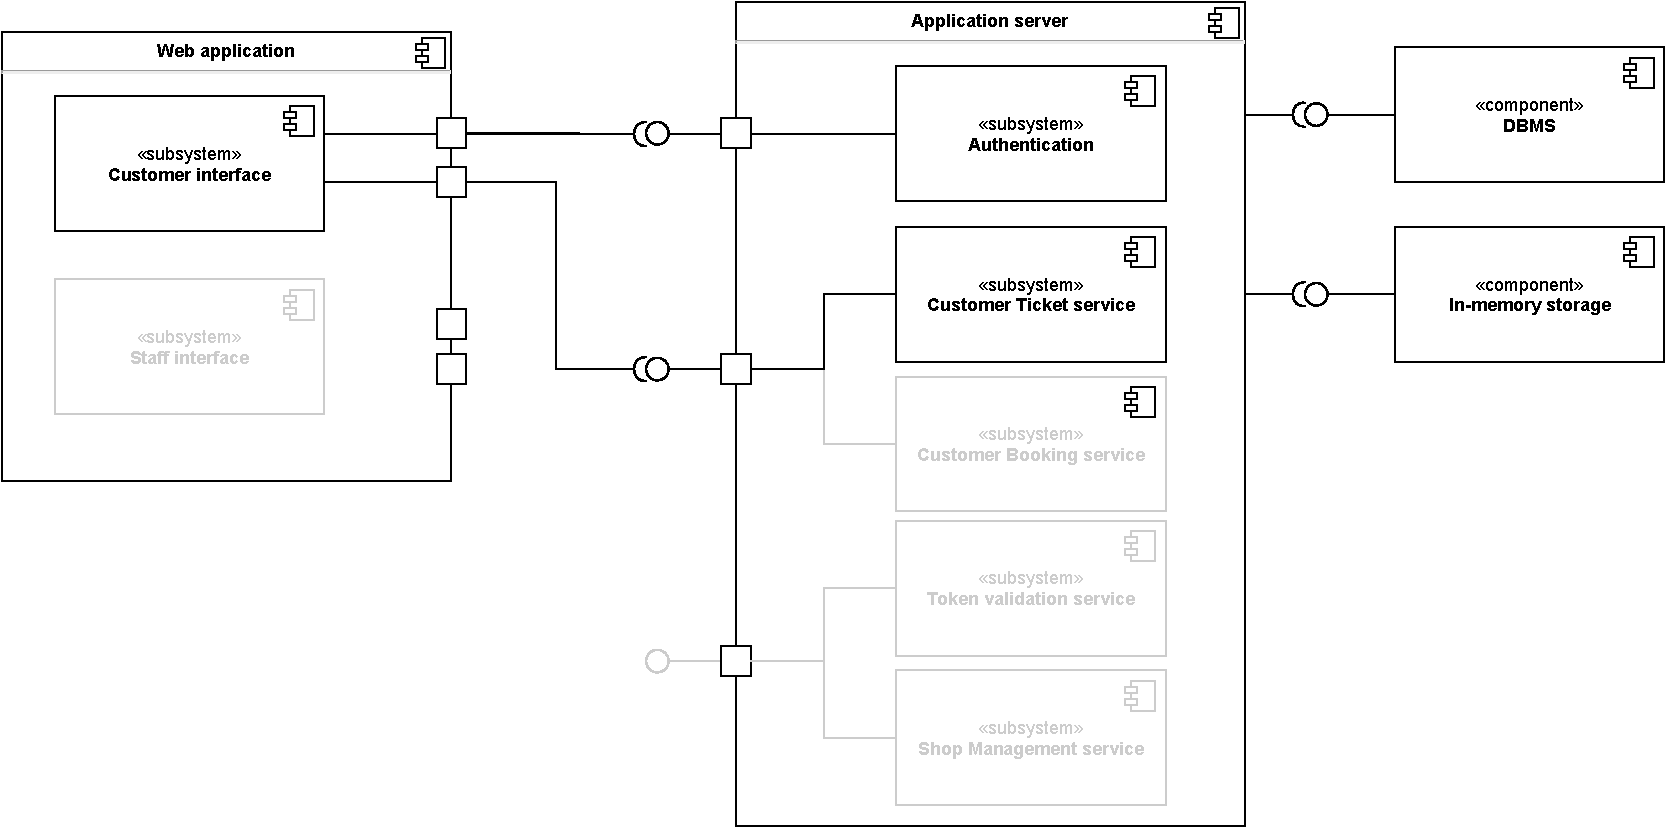
\includegraphics[width=0.9\textwidth]{Images/component2_tb.pdf}
\end{figure}

The system should be written starting from a subset of functionality implemented from the start to the end. Then the other functionalities will be added alongside what was already written.

The first thing to be programmed should be the authentication and account creation, interfacing with the DBMS and the memory storage and exposing a minimal API. By doing so, the system can reach a working state with reduced functionality, \emph{but \todo{structurally complete}} with reduced overall complexity. Then other components can rely on the existing structure for integration.

The Ticket service should be implemented and integrated right after the Authentication, adding part of the core functionality.

The web application can be developed in parallel by referencing the proposed REST API for the first stages of development.

At this point a partially working version of the system is complete and can be \todo{checked in  with stakeholders}

The next components to be created and integrated should be the Staff interface with associated Token Validation service, then the Booking service and connection to the Search engine and then the Shop management service. The Search engine and Maps service  interfaces can be added in parallel after the first working version, since they have essentially zero coupling to the other parts of the system.

\subsection{Testing plan}